\documentclass[12pt,a4paper]{report}

\usepackage{float}
\usepackage{listings, listings-rust}
\usepackage{xcolor}
\usepackage{minted}

\definecolor{GrayCodeBlock}{RGB}{241,241,241}
\definecolor{BlackText}{RGB}{110,107,94}
\definecolor{RedTypename}{RGB}{182,86,17}
\definecolor{GreenString}{RGB}{96,172,57}
\definecolor{PurpleKeyword}{RGB}{184,84,212}
\definecolor{GrayComment}{RGB}{170,170,170}
\definecolor{GoldDocumentation}{RGB}{180,165,45}

\lstdefinelanguage{rust}
{
    columns=fullflexible,
    numbers=left,
    stepnumber=1,
    keepspaces=true,
    frame=lines,
    % framesep=0pt,
    % framerule=1pt,
    framexleftmargin=4pt,
    framexrightmargin=4pt,
    framextopmargin=5pt,
    framexbottommargin=3pt,
    xleftmargin=4pt,
    xrightmargin=4pt,
    % backgroundcolor=\color{GrayCodeBlock},
    basicstyle=\ttfamily\color{BlackText},
    keywords={
        true,false,
        unsafe,async,await,move,
        use,pub,crate,super,self,mod,
        struct,enum,fn,const,static,let,mut,ref,type,impl,dyn,trait,where,as,
        break,continue,if,else,while,for,loop,match,return,yield,in
    },
    keywordstyle=\color{PurpleKeyword},
    ndkeywords={
        bool,u8,u16,u32,u64,u128,i8,i16,i32,i64,i128,char,str,
        Self,Option,Some,None,Result,Ok,Err,String,Box,Vec,Rc,Arc,Cell,RefCell,HashMap,BTreeMap,
        macro_rules
    },
    ndkeywordstyle=\color{RedTypename},
    comment=[l][\color{GrayComment}\slshape]{//},
    morecomment=[s][\color{GrayComment}\slshape]{/*}{*/},
    morecomment=[l][\color{GoldDocumentation}\slshape]{///},
    morecomment=[s][\color{GoldDocumentation}\slshape]{/*!}{*/},
    morecomment=[l][\color{GoldDocumentation}\slshape]{//!},
    morecomment=[s][\color{RedTypename}]{\#![}{]},
    morecomment=[s][\color{RedTypename}]{\#[}{]},
    stringstyle=\color{GreenString},
    string=[b]"
}

\lstdefinelanguage{JavaScript}{
  keywords={typeof, new, true, false, catch, function, return, null, catch, switch, var, if, in, while, do, else, case, break, let, for, of, void, const},
  keywordstyle=\color{PurpleKeyword}\bfseries,
  ndkeywords={class, export, boolean, throw, implements, import, this},
  ndkeywordstyle=\color{RedTypename}\bfseries,
  identifierstyle=\color{BlackText},
  sensitive=false,
      comment=[l][\color{GrayComment}\slshape]{//},
  morecomment=[s]{/*}{*/},
  stringstyle=\color{GreenString}\ttfamily,
      basicstyle=\ttfamily\color{BlackText},
  % backgroundcolor=\color{GrayCodeBlock},
    columns=fullflexible,
    numbers=left,
    stepnumber=1,
    keepspaces=true,
    frame=lines,
    framexleftmargin=4pt,
    framexrightmargin=4pt,
    framextopmargin=5pt,
    framexbottommargin=3pt,
    xleftmargin=4pt,
    xrightmargin=4pt,
  morestring=[b]',
  morestring=[b]"
}

\lstdefinelanguage{GDB}{
  keywords={gdb},
  keywordstyle=\color{PurpleKeyword}\bfseries,
  ndkeywords={class, export, boolean, throw, implements, import, this},
  ndkeywordstyle=\color{RedTypename}\bfseries,
  identifierstyle=\color{BlackText},
  sensitive=false,
      comment=[l][\color{GrayComment}\slshape]{//},
  morecomment=[s]{/*}{*/},
  stringstyle=\color{GreenString}\ttfamily,
      basicstyle=\ttfamily\color{BlackText},
    columns=fullflexible,
    numbers=left,
    stepnumber=1,
    keepspaces=true,
    frame=lines,
    framexleftmargin=4pt,
    framexrightmargin=4pt,
    framextopmargin=5pt,
    framexbottommargin=3pt,
    xleftmargin=4pt,
    xrightmargin=4pt,
  morestring=[b]',
  morestring=[b]"
}

\usepackage[utf8]{inputenc} % pentru suport diacritice
\usepackage[english, romanian]{babel} % setări pentru limba română 
\renewcommand\familydefault{\sfdefault} % sans serif

\usepackage[margin=2.54cm]{geometry}	% dimensiuni pagină și margini
\usepackage{graphicx} % support the \includegraphics command and options

% formatting sections and subsections
\usepackage{textcase}
\usepackage[titletoc, title]{appendix}
\usepackage{titlesec}
\titleformat{\chapter}{\large\bfseries\MakeUppercase}{\thechapter}{2ex}{}[\vspace*{-1.5cm}]
\titleformat*{\section}{\large\bfseries}
\titleformat*{\subsection}{\large\bfseries}
\titleformat*{\subsubsection}{\large\bfseries}

\usepackage{chngcntr}
\counterwithout{figure}{chapter} % no chapter number in figure labels
\counterwithout{table}{chapter} % no chapter number in table labels
\counterwithout{equation}{chapter} % no chapter number in equation labels

\usepackage{booktabs} % for much better looking tables
\usepackage{url} % Useful for inserting web links nicely
\usepackage[bookmarks,unicode,hidelinks]{hyperref}

\usepackage{array} % for better arrays (eg matrices) in maths
\usepackage{paralist} % very flexible & customisable lists (eg. enumerate/itemize, etc.)
\usepackage{verbatim} % adds environment for commenting out blocks of text & for better verbatim
\usepackage{subfig} % make it possible to include more than one captioned figure/table in a single float
\usepackage{enumitem}
\setlist{noitemsep}

%%% HEADERS & FOOTERS
\usepackage{fancyhdr}
\pagestyle{empty}
\renewcommand{\headrulewidth}{0pt}
\renewcommand{\footrulewidth}{0pt}
\lhead{}\chead{}\rhead{}
\lfoot{}\cfoot{\thepage}\rfoot{}


\newcommand{\HeaderLineSpace}{-0.25cm}
\newcommand{\UniTextRO}{UNIVERSITATEA POLITEHNICA DIN BUCUREȘTI \\[\HeaderLineSpace] 
FACULTATEA DE AUTOMATICĂ ȘI CALCULATOARE \\[\HeaderLineSpace]
DEPARTAMENTUL DE CALCULATOARE\\}
\newcommand{\DiplomaRO}{PROIECT DE DIPLOMĂ}
\newcommand{\AdvisorRO}{Coordonator științific:}
\newcommand{\BucRO}{BUCUREȘTI}

\newcommand{\UniTextEN}{UNIVERSITY POLITEHNICA OF BUCHAREST \\[\HeaderLineSpace]
FACULTY OF AUTOMATIC CONTROL AND COMPUTERS \\[\HeaderLineSpace]
COMPUTER SCIENCE AND ENGINEERING DEPARTMENT\\}
\newcommand{\DiplomaEN}{DIPLOMA PROJECT}
\newcommand{\AdvisorEN}{Thesis advisor:}
\newcommand{\BucEN}{BUCHAREST}

\newcommand{\frontPage}[6]{
\begin{titlepage}
\begin{center}
{\Large #1}  % header (university, faculty, department)
\vspace{50pt}
\begin{tabular}{p{6cm}p{4cm}}

\includegraphics[scale=0.8]{pics/upb-logo.jpg} &
	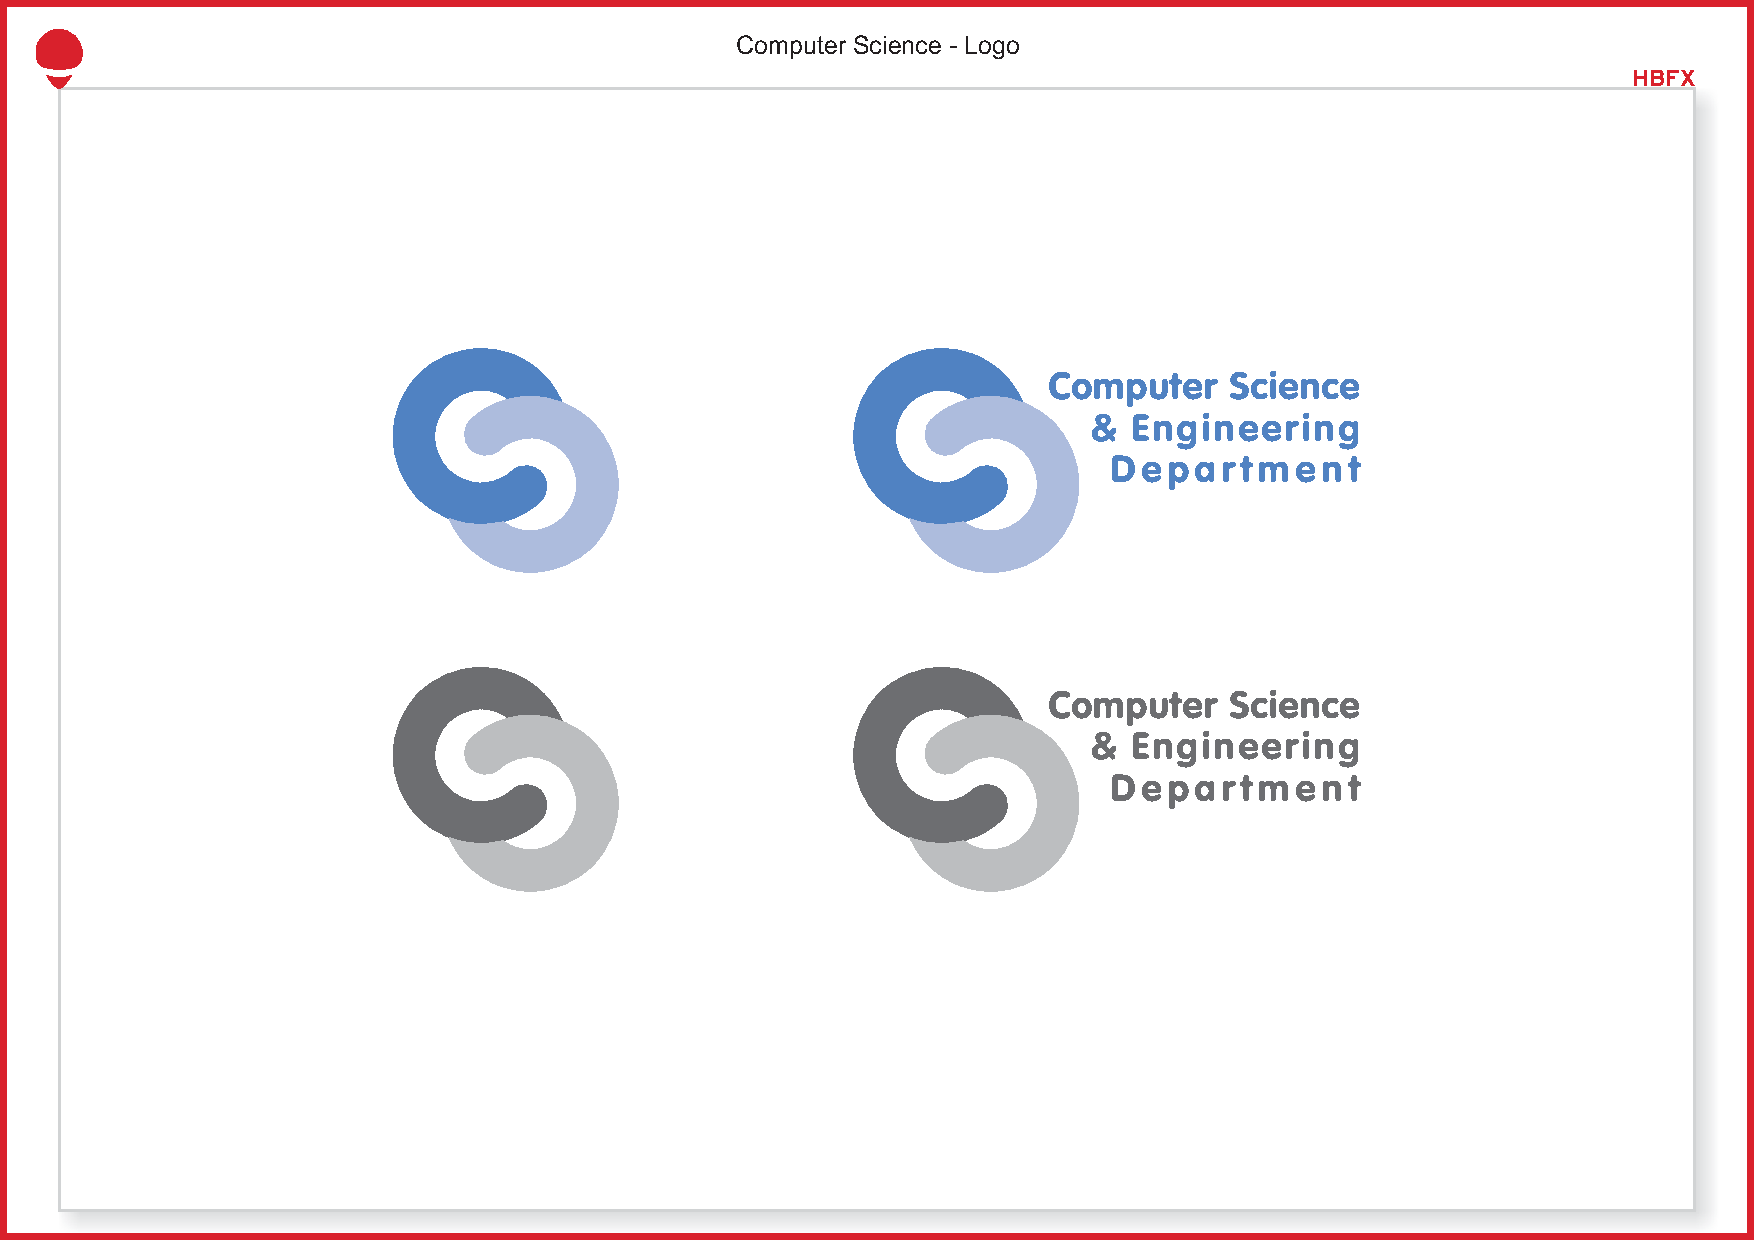
\includegraphics[scale=0.5,trim={14cm 11cm 2cm 5cm},clip=true]{pics/cs-logo.pdf}
\end{tabular}

\vspace{105pt}
{\Huge #2}\\                           % diploma project text
\vspace{40pt}
{\Large #3}\\ \vspace{0pt}  % project title
{\Large #4}\\                          % project subtitle
\vspace{40pt}
{\LARGE \Name}\\                   % student name
\end{center}
\vspace{60pt}
\begin{tabular*}{\textwidth}{@{\extracolsep{\fill}}p{6cm}r}
&{\large\textbf{#5}}\vspace{10pt}\\      % scientific advisor
&{\large \Advisor}                                    % advisor name
\end{tabular*}
\vspace{20pt}
\begin{center}
{\large\textbf{#6}}\\                                % bucharest
\vspace{0pt}
{\normalsize \Year}
\end{center}
\end{titlepage}
}

\newcommand{\frontPageRO}{\frontPage{\UniTextRO}{\DiplomaRO}{\ProjectTitleRO}{\ProjectSubtitleRO}{\AdvisorRO}{\BucRO}}
\newcommand{\frontPageEN}{\frontPage{\UniTextEN}{\DiplomaEN}{\ProjectTitleEN}{\ProjectSubtitleEN}{\AdvisorEN}{\BucEN}}

\linespread{1.15}
\setlength\parindent{0pt}
\setlength\parskip{.28cm}

%% Abstract macro
\newcommand{\AbstractPage}{
\begin{titlepage}
\textbf{\large SINOPSIS}\par
\AbstractRO\par\vfill
\textbf{\large ABSTRACT}\par
\AbstractEN \vfill
\end{titlepage}
}

%% Thank you macro
\newcommand{\ThanksPage}{
\begin{titlepage}
{\noindent \large\textbf{MULȚUMIRI}}\\
\Thanks
\end{titlepage}
}

%%%%%%%%%%%%%%%%%%%%%%%%%%%%%%%%%%%%%%%%%%%%%%%%%%   
%%
%%          End of template definitions
%%   
%%%%%%%%%%%%%%%%%%%%%%%%%%%%%%%%%%%%%%%%%%%%%%%%%%

\newcommand{\worktype}[1]{[\textit{#1}] }
\newcommand{\dezvoltare}{\worktype{Dezvoltare de produs}}
\newcommand{\cercetare}{\worktype{Cercetare}}
\newcommand{\ambele}{\worktype{Ambele}}

%%
%%   Campurile de mai jos trebuie modificate de autor. Modificati doar continutul, nu si numele fiecarei definitii
%%
\newcommand{\ProjectTitleRO}{Portarea unui sistem de operare pentru microprocesoare pe o platformă WebAssembly}
\newcommand{\ProjectTitleEN}{Porting an Embedded Operating System on WebAssembly}
\newcommand{\Name}{Niță Irina-Cristina}
\newcommand{\Advisor}{Prof. dr. ing. Răzvan Victor Rughiniș}
\newcommand{\Year}{2024}

% Setări document
\title{Proiect de diplomă}
\author{\Name}
\date{\Year}

%%
%%   Campurile aferente rezumatului
%%
\newcommand{\AbstractRO}{Sinopsisul proiectului are rol de introducere, conținând atât o descriere pe scurt a problemei abordate cât și o enumerare sumară a rezultatelor și a concluziilor. Se recomandă ca sinopsisul să fie redactat într-un limbaj accesibil unei persoane nefamiliarizate cu domeniul, dar în același timp destul de specific pentru a oferi rapid o vedere de ansamblu asupra proiectului prezentat.
Sinopsisul proiectului va fi redactat atât în română cât și în engleză. Ca dimensiunea recomandată aceasta secțiune va avea maxim 200 de cuvinte pentru fiecare variantă. Împreună, ambele variante se vor încadra într-o singură pagină.}

\newcommand{\AbstractEN}{The abstract has an introductory role and should engulf both a brief description of the issue at hand, as well as an overview of the obtained results and conclusions. The abstract should be formulated such that even somebody that is unfamiliar with the projects’ domain can grasp the objectives of the thesis while, at the same time, retaining a specificity level offering a bird’s eye view of the project.
The projects’ abstract will be elaborated in both Romanian and English. The recommended size for this section is limited to 200 words for each version. Together, both versions will fit in one page.}

%%
%%   Campurile aferente paginii de multumiri
%%
\newcommand{\Thanks}{(opțional) Aici puteți introduce o secțiunea specială de mulțumiri / acknowledgments. }

\begin{document}

\frontPageRO
\frontPageEN

\begingroup
\linespread{1}
\tableofcontents
\endgroup

\AbstractPage

% poate fi comentata sau stearsa
\ThanksPage

\selectlanguage{english}
\chapter{Introduction}\pagestyle{fancy}

\section{Context}

% WASM: Keywords: Viable, Sandbox, Platform Independent, Portable, Ubiquitous
% TockOS: Keywords: Embedded, Rust, Hybrid in terms of kernel
As microcontrollers (MCUs) are increasingly becoming more advanced,
embedded software developers have the ability to leverage the hardware to build
real-time systems that can run multiple applications simultaneously.
Coordinating multiple tasks on a platform with limited resources, such as memory,
implies running a memory-efficient operating system with, at least, a scheduler.
Due to good performance and low memory footprint, most systems are written in low-level
languages, usually C/C++, but are prone to memory-related security vulnerabilities.

Tock is an operating system written in Rust, a low-level systems programming language similar to C, but memory-safe.
As illustrated in \autoref{fig:tock},
the Rust feature seen most prominently in the Tock codebase is the separation between
safe and unsafe code. The operating system kernel and microcontroller-specific peripheral drivers
are considered "trusted" code, i.e. unsafe Rust is allowed; the drivers that define the application
program interfaces (APIs) for user applications are deemed "untrusted", i.e. unsafe Rust is forbidden.

% TODO: Image of Tock here

\begin{figure}[H]
\centering
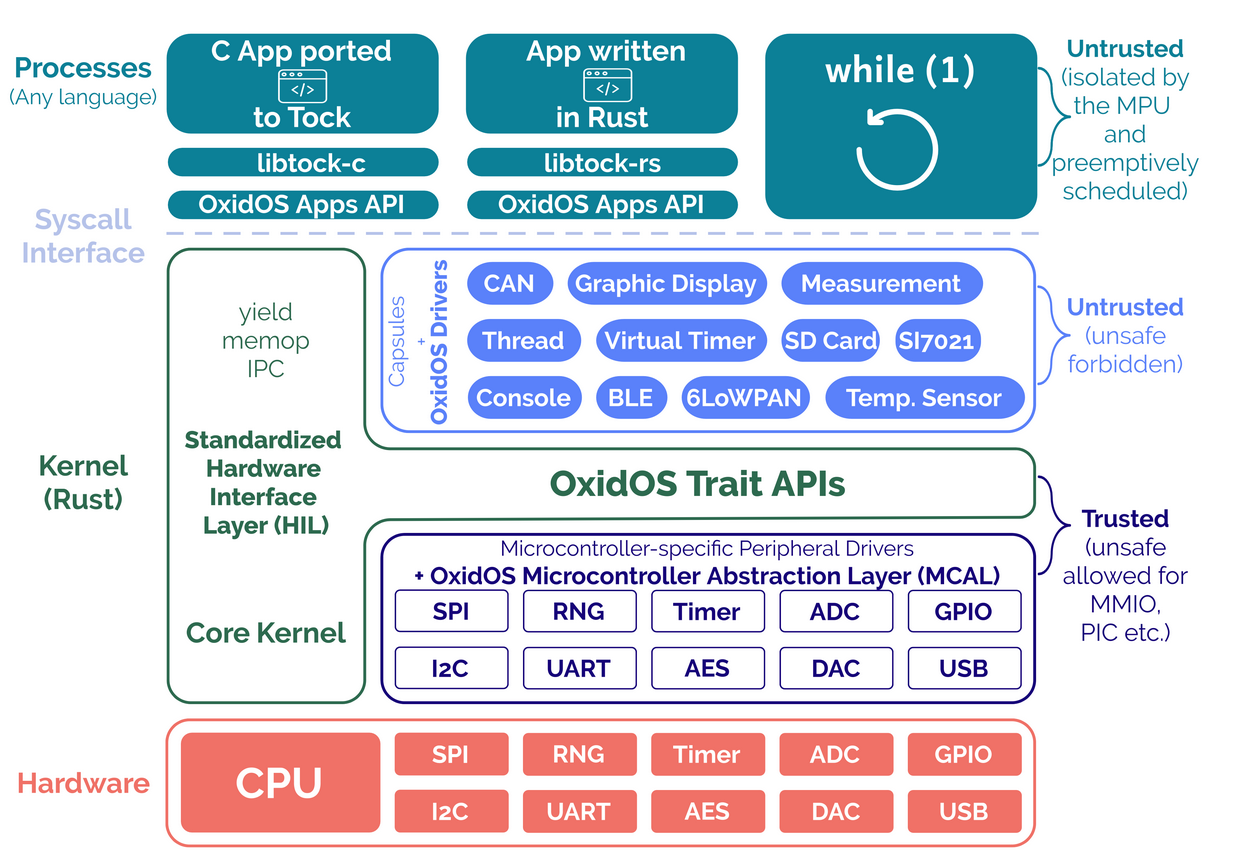
\includegraphics[scale=0.65]{pics/oxidos-stack.png}
  \caption[Tock operating system software stack]{Tock operating system software stack}
  \label{fig:tock}
\end{figure}

The abstraction acquired in Tock through Rust generics and traits (similar to "interfaces"
in other languages) ensures portability, allowing the drivers and kernel implementation to
remain agnostic regarding the hardware platform they are running on. Therefore, Tock could
eventually run on most targets if the minimum set of requirements for booting up the
kernel on a platform is met. The support list, alongside the modern MCUs' most prevalent
architectures (e.g. RISC-V, ARM), could include a more unusual choice, WebAssembly
(Wasm).

% TODO: Image of Wasm here
\begin{figure}[H]
\centering
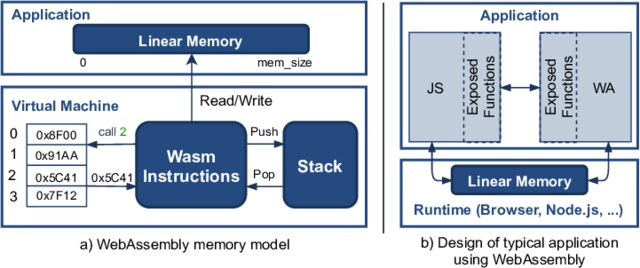
\includegraphics[scale=1.65]{pics/WebAssembly-high-level-architecture_W640-2.jpg}
  \caption[WebAssembly high-level architecture]{WebAssembly high-level architecture}
  \label{fig:wasm}
\end{figure}

WebAssembly is a binary instruction format that emerged from the Web's demand for interoperability with other programming languages, with the same or increased speed performance as native JavaScript. Through the portability of the Wasm compilation target, code written in low-level languages (C, C++ or Rust) is able to run on any platform, either Web embedded (in browser, e.g. Mozilla, or a JavaScript virtual machine, e.g. node.js) or in a non-Web environment (custom WebAssembly runtimes, e.g. Wasmtime). So, building Wasm support for an operating system inherently can be translated to building multi-platform support at once.

% TODO: Unicorn (that is also wasm)

\section{Motivation and Problem Statement} 

The main goal of this thesis is to provide a virtual environment for Tock by running the operating system on a transparent platform. The system is currently supported on Cortex-M and RISC-V chips; thus, it can only be tested on a physical board or an emulated one with significant restrictions. Adding support for WebAssembly eliminates the need for a hardware emulator, e.g., Qemu, during the software development process.

Part of Tock's porting process on Wasm consists of handling user applications through loading process binaries and handling system calls. Although the applications are not technically part of the operating system, Tock's virtualization process implies support for the whole environment, including user applications.

As of right now, the ability to run Tock locally is limited. The absence of physical hardware implies either using an architecture emulator, which eliminates the idea of a simulation of peripherals, or third-party simulation software, e.g., WokWi, which is suitable for running a single embedded application on a well-known MCU but is restricted in terms of platforms it simulates and is not tailored to the operating system.

\section{Proposed Solution}

This thesis proposes an ecosystem incorporating support and tooling for developing Tock on users' machines, eliminating the necessity for physical hardware. The virtual platform comprises two components: the WebAssembly operating system kernel and the user applications that can be loaded into the platform's virtual flash memory.

In addition to UART or timers, the simulation of hardware peripherals can extend to graphical-based interaction through communication between the user interface and the peripherals' behavior description protocol.

Tock's process console, a small shell over serial communication (UART), is available by simulating hardware peripherals for more debugging support. Users can access it via a terminal emulator to inspect the kernel and control userspace processes.

The platform provides debugging support for the simulated environment to imitate the developing process on physical MCUs. The debugger stub supports stepping through code, adding breakpoints, and getting information about registers and internal variables' values.

\section{Thesis Structure}

This paper begins with the background chapter, bringing the discussion into a theoretical context by providing introductory information on the technologies and terminology further used in the thesis.

The following chapter defines the architecture design for the system components at a higher level, remaining agnostic in implementation to the fullest extent possible. Therefore, the chapter on implementation details describe the methods and technologies used in creating this project. 

The chapter on related work presents the Wokwi platform, similar idea to this thesis, but not tailored for a specific operating system or runtime. The evaluation chapter describes the validation process of the platform. 
The thesis ends with a conclusion on the results acquired and a discussion on further improvements.

\chapter{Background}\pagestyle{fancy}

\section{Rust}

Rust is a remarkable programming language because it provides memory-safety without using a garbage collector; besides memory, Rust stands out by being thread-safe, preventing data races. These compile-time features make it a favorable alternative to other candidate low-level programming languages in embedded systems, in addition to the fact that it can be used to extend existing legacy codebases written in C due to its interoperability with the language. 

\subsection{Types, traits and generics}

As a low-level programming language that is designed with characteristics comprising multiple programming paradigms. In spite of comparing traits to OOP's interfaces, the concept of classes or inheritence is not associated with Rust. Instead, the multi-paradigm programming languages provides data types alongside primitives, similar to C, using structs or enums.

Traits define abstraction in Rust and comprise of methods, types or constants definitions. Any type can implement a trait, as long as either one is defined in the current crate, e.g. a primitive type can't implement a trait exported from the std crate outside of its definition scope.

Generics are used in functions' or structs' definitions to act as "placeholders" for multiple concrete data types. The generic types are a compile-time features, such as for each concrete data type that is used to replace the generic, a copy of the definition will be created by the compiler. Generics can be trait-bounds, as in they are restricted to types that implement certain traits.

\subsection{Ownership and borrow checker}

The primary characteristics that make Rust a memory-safe language are the ownership system and the borrow checker.

The ownership system is used by the compiler to know when to safely drop a variable's value when its owner goes out of scope, so a variable can only have one owner at a time. This system works differently for heap and stack allocated variables, because variables on the stack are copyable, therefore, what can seem to result in a compilation error, might not due to the fact that the compiler is capable enough to copy the variable's value instead of moving it out of scope. Copyable types are defined through the marker trait Copy, and its implemented by all primitive types.

The borrow checker alludes to references, i.e. borrowed ownership. Rust contains two types of references: mutable and immutable. There can only exist one mutable reference and no immutable references to a variable at a time, or multiple immutable references and no mutable reference to a variable at a time. The principle is that multiple reads of the same variable won't affect its value, so it's thread-safe and allowed, but concurrent writes might result in undefined behavior, so it's forbidden. Borrowed variables can not be deallocated by the scope where the ownership was borrowed, so after the end of that scope, ownership is returned.

\subsection{Unsafe Rust}

Rust actually comprises a set of two programming languages: safe Rust and unsafe Rust. The previous section detailed about the programming language's core principles on memory-safety; these still apply to unsafe Rust. The underlying language is considered unsafe because it stops the compiler from executing some additional checks, e.g. deferencing a raw pointer or having a mutable static variable. These features are needed in low-level programming, explicitly developing embedded software, e.g. writing a value to a memory-mapped register.

\section{Tock}

Tock is an embedded operating system for low-power microcontrollers written in Rust. The Tock kernel is modular and comprises abstraction layers through Rust traits. As previously defined, Tock separates software-defined privilege rings by trustfulness, where allowing unsafe code is deemed as trusting the code. In other words, the closer the layer to necessary bare-metal programming, e.g., modifying registers, the more "trusted" the module. From a higher-level perspective, the operating system incorporates four components: the hardware interface layer, the microcontroller abstraction layer, the core kernel and the capsules.

\newpage
\subsection{Hardware Interface Layer (HIL)}

This layer of abstraction acts as glue between drivers and microcontroller-specific peripherals. The HIL modules expose mostly traits that a driver needs for a peripheral to implement. Therefore, the drivers are unaware of a peripheral's memory-mapped register values but know that it can serve the functionality the driver needs to integrate, regardless of how the functions are implemented.

\begin{lstlisting}[caption={Trait for configuring UART peripherals},label={lst:cfg-trait},language=Rust]
// kernel/src/hil/uart.rs

/// Trait for configuring a UART.
pub trait Configure {
    /// Returns Ok(()), or
    /// - OFF: The underlying hardware is currently not available,
    ///         perhaps because it has not been initialized or in
    ///         the case of a shared hardware USART controller because
    ///         it is set up for SPI.
    /// - INVAL: Impossible parameters (e.g. a `baud_rate` of 0)
    /// - ENOSUPPORT: The underlying UART cannot
    ///               satisfy this configuration.
    fn configure(&self, params: Parameters) -> Result<(), ErrorCode>;
}
\end{lstlisting}

Because the configuration of the UART peripheral (word length, stop bits, parity bits, baud rate) is a protocol standard relevant to all MCUs that support serial communication, the Configure trait is found necessary and generic for what would be defined as a UART peripheral. This generalization principle applies likewise to the Transmit and Receive trait, as the peripheral is required to handle both ends of the communication to conform to the UART protocol.

\begin{lstlisting}[caption={Blanket trait encorporating the UART functionalities},label={lst:uart-trait},language=Rust]
// kernel/src/hil/uart.rs

pub trait Uart<'a>: Configure + Transmit<'a> + Receive<'a> {}
impl<'a, T: Configure + Transmit<'a> + Receive<'a>> Uart<'a> for T {}
\end{lstlisting}

\newpage
\subsection{Microcontroller Abstraction Layer (MCAL)}

The microcontroller abstraction layer incorporates multiple crates defining supported chips by Tock. Microcontroller support can be divided in two components: peripherals and chip support which comprises in addition the interrupt service. The chip's peripherals are configured using MCU-specific memory-mapped registers. The chip support component defines how the chip encapsulates both architecture-specific and peripheral-specific tasks, e.g., handling pending interrupts. Both these categories of implementation are used to implement the hardware interface layer's defined traits.

\begin{lstlisting}[caption={Configure trait implementation for Uart peripheral struct},label={lst:uart-impl},language=Rust]
// kernel/src/hil/uart.rs

pub trait Uart<'a>: Configure + Transmit<'a> + Receive<'a> {}
impl<'a, T: Configure + Transmit<'a> + Receive<'a>> Uart<'a> for T {}
\end{lstlisting}

\subsection{Capsules}

Capsules are another name for device drivers in Tock. The capsule implementation leverages the programming language's generics for adding transparency in terms of the peripheral that it encapsulates. These drivers rely heavily on the hardware interface layer trait-bounds of their definition's generics.

\begin{lstlisting}[caption={Console capsule struct definition},label={lst:console-strct},language=Rust]
// kernel/src/hil/uart.rs

pub trait Uart<'a>: Configure + Transmit<'a> + Receive<'a> {}
impl<'a, T: Configure + Transmit<'a> + Receive<'a>> Uart<'a> for T {}
\end{lstlisting}

\subsection{Tock Binary Format (TBF)}

Each application binary must be in Tock Binary Format (TBF) before being loaded in the operating system. The TBF standard defines a header (protected region), from which the kernel can interpret information regarding the binary, e.g. the size, the start symbol. Additionally, it may include also a footer and padding. 

\newpage
\section{WebAssembly}

WebAssembly is a low-level language similar to assembly designed for a stack-based virtual machine. Along with platform independence, it provides isolation and security features, e.g., a protected call stack, making Wasm a favorable option for running sandboxed applications. However, it can't entirely cover the undefined behavior of programming languages like C, so picking a memory-safe language like Rust for this compilation target equips an additional layer of security.

Wasm's primary component is the module, which comprises functions, types, variable definitions, imports of other modules, and exports. The latter two are central to the programming language's interoperability.

As mentioned in the paper's introduction, WebAssembly can have different runtime, but running Wasm in a non-web embedded environment is beyond the scope for this thesis.

\begin{lstlisting}[caption={WebAssembly instantiation in JavaScript},label={lst:wasm-inst},language=JavaScript]
// kernel/src/hil/uart.rs

pub trait Uart<'a>: Configure + Transmit<'a> + Receive<'a> {}
impl<'a, T: Configure + Transmit<'a> + Receive<'a>> Uart<'a> for T {}
\end{lstlisting}

JavaScript, alongside its type-safe extended language, TypeScript, can instantiate and run Wasm code out of the box, alongside providing imports to the instance, using the WebAssembly object.  

\section{Unicorn.js}

Unicorn Engine is a lightweight CPU emulator framework based on Qemu. The core is written in pure C and supports multiple binding languages. The emulator API allows users to modify registers, allocate memory for the virtual CPU, or define hooks for specific instructions or events.

\begin{lstlisting}[caption=Memory fault hook using Unicorn.js\protect\footnotemark,label={lst:unicorn-mem-fault},language=JavaScript]
// Hook for unmapped memory fault.
var unicorn = new uc.Unicorn(CpuArch.ARCH_ARM, CpuMode.MODE_THUMB);
// hook_fault is a function previously defined.
unicorn.hook_add(HookType.HOOK_MEM_READ_UNMAPPED, hook_fault); 
\end{lstlisting}

The configurable event handlers are effectively the functionality that sets Unicorn Engine apart from Qemu since errors or interrupts
can be monitored and controlled by the emulator. The code chunk seen in Listing 2.3 showcases the simplicity of adding a hook to an error, as the common errors are already found as constants in the Unicorn API.

\footnotetext{To maintain type safety across the project, our virtual platform uses a TypeScript wrapper of the Unicorn.js package. Examples or references to Unicorn.js will inherently refer to the TypeScript port.}

\section{Remote GDB}

Due to resource limitations on embedded systems, debugging is done remotely from a host machine. The procedure requires a client that communicates through a debugger remote protocol with the embedded device and uses these packets to modify or investigate the state of the running program. The server executing on the embedded device to control and investigate the program's state is named a stub or an agent.

\begin{lstlisting}[caption=Initiating a remote connection on GDB,language=GDB]
(gdb) set architecture armv7e-m
(gdb) target remote 127.0.0.4:2000
\end{lstlisting}

Because of its extended documentation, this paper utilizes the GNU Debugger (GDB) and the GDB Serial Remote Protocol (RSP). Regardless of its name, the remote protocol supports more than direct serial connections, including UDP and TCP connections. The connection for the latter two is established by giving GDB the command "target remote" followed by the stub IP and port, separated by a colon.

\chapter{System Design and Architecture}

\section{WebAssembly kernel}

In order to simulate a physical MCU, the virtual microcontroller must have defined platform-specific peripherals. Currently, the simulator chip implements the functionality of four peripherals: timer, UART, GPIO, and CAN, which can be separated into two types of virtual peripherals:
the ones that can be dispatched to the user's system (timer, UART) and those that require simulation due to specific behaviors not directly found on one's local machine (UART, GPIO, CAN).

The serial communication peripheral falls into both categories due to the platform's portability, such as running on a medium that does not provide a terminal emulator for the UART messages to be forwarded to and visible to the user, e.g., a browser. The choice between forwarding to the system and simulating the peripheral is done at runtime, where the environment is on which the platform runs is selected.

Therefore, the system operates in two modes: in a local environment, where only the timers and serial communication are available, or in a simulated environment, where multiple peripherals can be accessed but require an agent to communicate the microcontroller's state.

\section{Hardware-emulated userland processes}

The userland applications are compiled to a Cortex-M4 target and run using a hardware emulator. Due to the operating system running in a Wasm virtual machine in a non-emulated environment, a context switch between the kernel and the user processes implies updating the context for the emulated MCU.

Tock's context switch implementations are defined (separately from the microcontroller abstraction layer) for each supported architecture and are primarily written in inline assembly. Thus, instead of directly using Thumbv7 instructions, the emulator acts as an additional layer. This interferes with the kernel in two situations: switching the execution from userspace to kernel space when the emulator must be paused from running and its context saved and switching the execution from kernel space to userspace when the emulator must be resumed and its context updated.

The debugger stub must have real-time access to read and modify the running user process's internals. For hardware-emulated applications, the stub is a server running concurrently with the application. Both threads share synchronized status buffers that contain information regarding registers, memory and breakpoints.

\chapter{Implementation details}

\section{Microcontroller support for virtual platform}

As a basis, the implementation of the microcontroller abstraction layer is required for the virtual MCU to support running Tock. This includes peripheral and interrupts service support through the implementation of HIL traits.

Due to WebAssembly's interoperability, an instance's modules can be included in other modules, regardless of the original pre-compilation programming language. The virtual chip's implementation leverages this aspect and glues Rust and TypeScript modules. 

The TypeScript functions included in the chip's implementation in Rust act as placeholders for what would have been memory-mapped registers in MCUs. In other words, they expose a connector between the chip's inner workings (for physical chips, this refers to the hardware, and for our virtual platform, it refers to the TypeScript simulator) and the program. Although external functions from other programming languages are unsafe to use, so is writing  to mutable static memory (mapped registers).

\begin{lstlisting}[caption=TypeScript functions imported in Rust from the gpio module, language=Rust]
// chips/deno/src/gpio.rs

/// Link the WebAssembly module.
#[link(wasm_import_module = "gpio")]
extern "C" {
    fn set_pin_state(port: usize, pin: usize, value: usize);
    fn get_pin_state(port: usize, pin: usize) -> usize;
    fn enable_interrupt(port: usize, pin: usize, edge: usize);
    // Other exposed functions...
}
\end{lstlisting}

The chip crate uses these exported functions to implement HIL traits, and the inner changes of the simulated platform remain transparent. 

The definitions of simulated peripherals are located in the TypeScript code.
The peripherals' state is shared and modified through an instance of a
WebSocket server communicating with an external client. Therefore, each time the client sends a packet updating the state of a peripheral, e.g., input-configured GPIO pin transitions edge, the inner state of a peripheral is updated. The pin example can be compared to a read-only data register that stores each pin's current state, mapping the bits to the corresponding GPIO pin numbers. The register is readable for the programmer (exported TypeScript function for getting a pin's state). However, the inner process is transparent (the instance's socket receives a packet, and the peripheral's state variable is updated).

The protocol used between the WebSocket server in the peripherals' implementation and the client is JSON-based. It contains the peripheral type, the peripheral-specific command, and the command payload. For state synchronization, the client and server updates are reciprocal.

The interrupt handling routine is similar to that of the physical chips. The TypeScript implementation contains the state of interrupts and exposes functions for clearing them upon firing. Setting an interrupt as pending is done by updating the inner buffers when receiving a packet payload that was previously configured as interrupt triggering, e.g., receiving a positive edge transition on a GPIO pin with interrupt enabled on any edge transition. Information about precisely the moment when these interrupts are set as pending will be further discussed in the following section as it relates to the kernel and puts it in a better context.

% // Other implementations...

% /// Implement the HIL Input trait for the virtual Pin.
% impl hil::gpio::Input for Pin<'_> {
%     fn read(&self) -> bool {
%         unsafe {
%             match get_pin_state(0, self.pinid as usize) {
%                 0 => false,
%                 _ => true,
%             }
%         }
%     }
% }

\section{Deno virtual board running the WebAssembly kernel}

In Tock's modularity-based design, the board's main function is separate from the chip's implementation. This crate defines the board's setup, e.g., the chip initialization, the scheduler configuration, the stack size, the maximum number of processes, and the supported drivers. After booting up the platform, the kernel's main loop can run.

For our platform, this crate is compiled to the Wasm compilation target and instantiated in a TypeScript file, serving as the virtual board's starting point. The Rust crate does not execute on its own but rather exposes the functions required for the board to run on the simulated platform, i.e., the setup function and the kernel loop function that needs ownership of the board defined in the crate.

\begin{lstlisting}[caption=Redefined kernel loop, language=JavaScript]
/**
 * Kernel's main loop
 */
function kernel_loop() {
  denoChip.kernelLoopBefore();
  denoChip.kernel.kernel_loop();
  denoChip.kernelLoopAfter();

  setTimeout(kernel_loop, 0);
}
\end{lstlisting}

As opposed to the usual kernel's main loop that runs directly after the setup in the Rust crate, this loop requires a routine before and after the execution. These additions are required because the operating system is running single-threadly in the same process as the peripherals' simulator\footnote{Tock is not running on top of a simulator, but it is running natively on a platform that also simulates its peripherals.}. 

\begin{lstlisting}[caption=Routine before the kernel's main loop, language=JavaScript]
/**
 * Function called before each kernel loop
 */
kernelLoopBefore(): void {
  for (const [_name, peripheral] of Object.entries(this.peripherals)) {
    peripheral.kernelLoopBefore();
  }
}
\end{lstlisting}

The routines call each peripheral's defined function. The before and after loop functions are exposed through the classes extending the Peripheral interface and apply to all simulated peripherals. The implementation for both heavily depends on the peripheral's purpose. However, the functions are generally accountable for setting the pending interrupts and updating the internal receiving buffer in case of the existence of one (e.g., UART, CAN).

This component is also responsible for loading the user application binaries into memory, reading the TBF file and writing its content to an internal buffer that serves as the virtual flash memory.

\section{Unicorn.js hardware-emulated user processes}

The user application binaries are executed by the Unicorn.js hardware emulator, which is instantiated inside the operating system kernel on the first context switch from kernelspace to userspace. The operating system is responsible for keeping and updating the context of the hardware emulator.

The context switch from kernelspace to userspace is done by resuming the emulator with the saved context from the previous run. The switch back is done by adding a hook in the emulator that handles each supervisor call (svc) instruction execution, this stops the current execution of the emulator and saves the svc number so that the appropriate system call is requested to the kernel.

The debugger stub starts its execution at same time with the emulator, but doesn't stop executing while switching context, as it will result in the GDB client interpreting it as an error and exiting\footnote{While the process yields, the debugger will be in a standby mode, so for some breakpoints it may take longer to reach.}. The debugging server runs as a TypeScript webworker concurrently with the application, sharing multiple Atomic state buffers. These buffers are synchronized with the application during execution, being updated for each instruction. The stub updates the values on received packets, e.g. command for adding a breakpoint adds the instruction address to an internal buffer that is used for instructions to be compared against and stopped when matched.

RSP defines three types of packets, or commands, that the client (GDB) sends to the server (stub): the ones that require acknowledgement, those that don't, and those that need to return a certain value. For the packets that do require a response, either an acknowledgment or a payload, data loss might result in GDB errors or loosing connection and the client exiting. That's why a protocol like UDP isn't considered suitable for the implementation of the GDB server, therefore, the GDB stub uses TCP sockets for communicating through packets.

\chapter{Related work}

\section{Wokwi platform}

Wokwi is an open-source web application for simulation of embedded device and IoT (Internet of things) projects. It provides an accesible user interface for connecting devices and writing code for MCUs. The platform internals provides a MCU simulator for each of the supported development boards. For performance improvmenet, each simulator runs on client-side and is written in TypeScript from scratch, without involving a third-party hardware emulator written in another language exported.

This platform supports simulating programs written in multiple programming languages, such as C, Rust and MicroPython. Besides being a browser-based platform, Wokwi provides Visual Studio Code support through an extension used for development.

\begin{figure}[H]
\centering
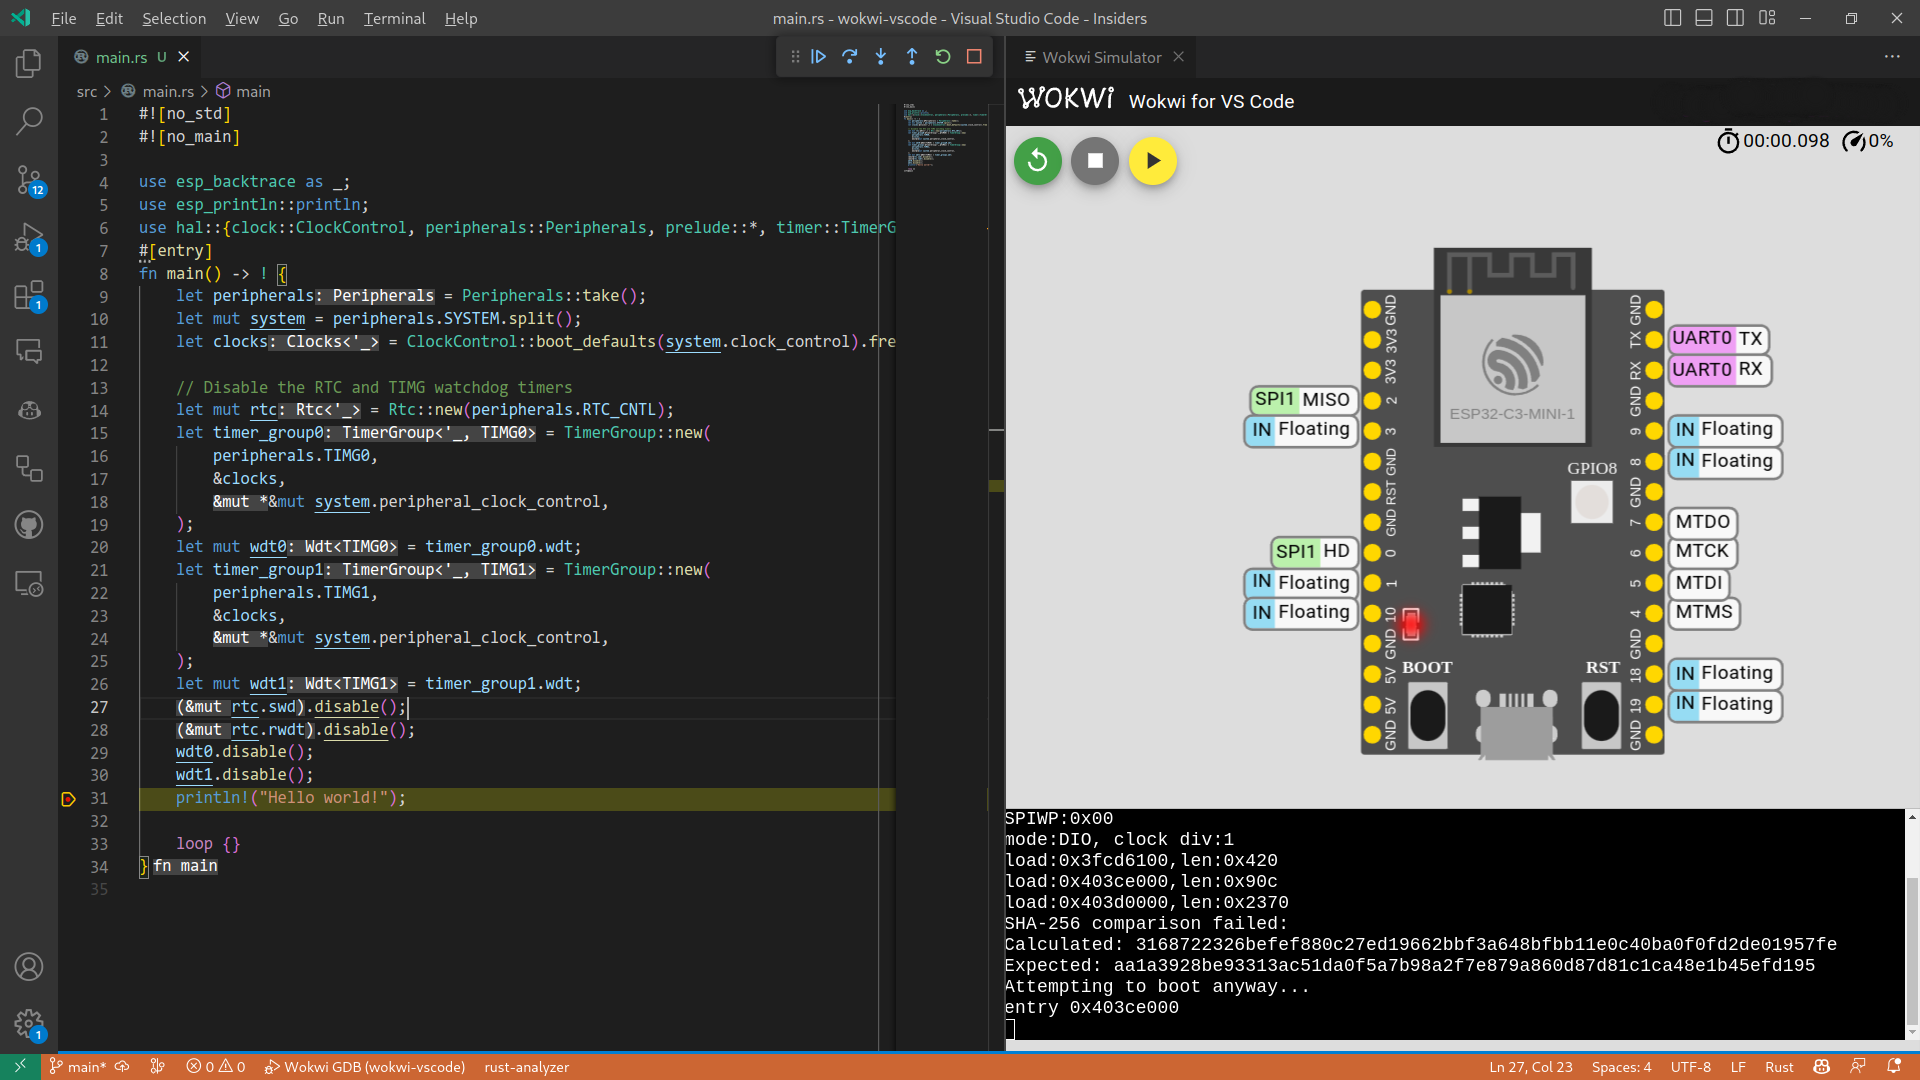
\includegraphics[scale=0.20]{pics/wokwi-vscode.png}
  \caption[Wokwi platform on Visual Studio Code]{Wokwi platform on Visual Studio Code}
  \label{fig:platform}
\end{figure}

\chapter{Evaluation}

\section{Development environment integration}

In order for the virtual platform to be evaluated as an ecosystem of development tools for Tock, integration with a text editor and graphical interfaces for the interaction with the simulated MCU's peripherals should be possible.

The text editor of choice for this demonstration was the open-source version of Microsoft's Visual Studio Code, which ranks high in experience customisability, with multiple possibilities of adding external features and add-ons.

\subsection{Visual simulated peripherals}

Simple electrical components like LEDs and switches are automatically connected to the WebSocket server of the board when assigned to one of the microcontroller's GPIO pins.

For the simulated peripherals to be validated, these components must behave in according to the application. When pressing or releasing a switch connected to an input pin, an interrupt must be fired on the virtual chip (the configuration of the kernel defines both edges as interrupt-triggering).
When the application sets the Led driver to "on", the LED connected to the corresponding output pin must illuminate, and the opposite when set to low.

This behavior was tested by loading a C application binary that turns on a LED for the corresponding switch pressed, and turns it off when the switch is released.

\begin{figure}[H]
\centering
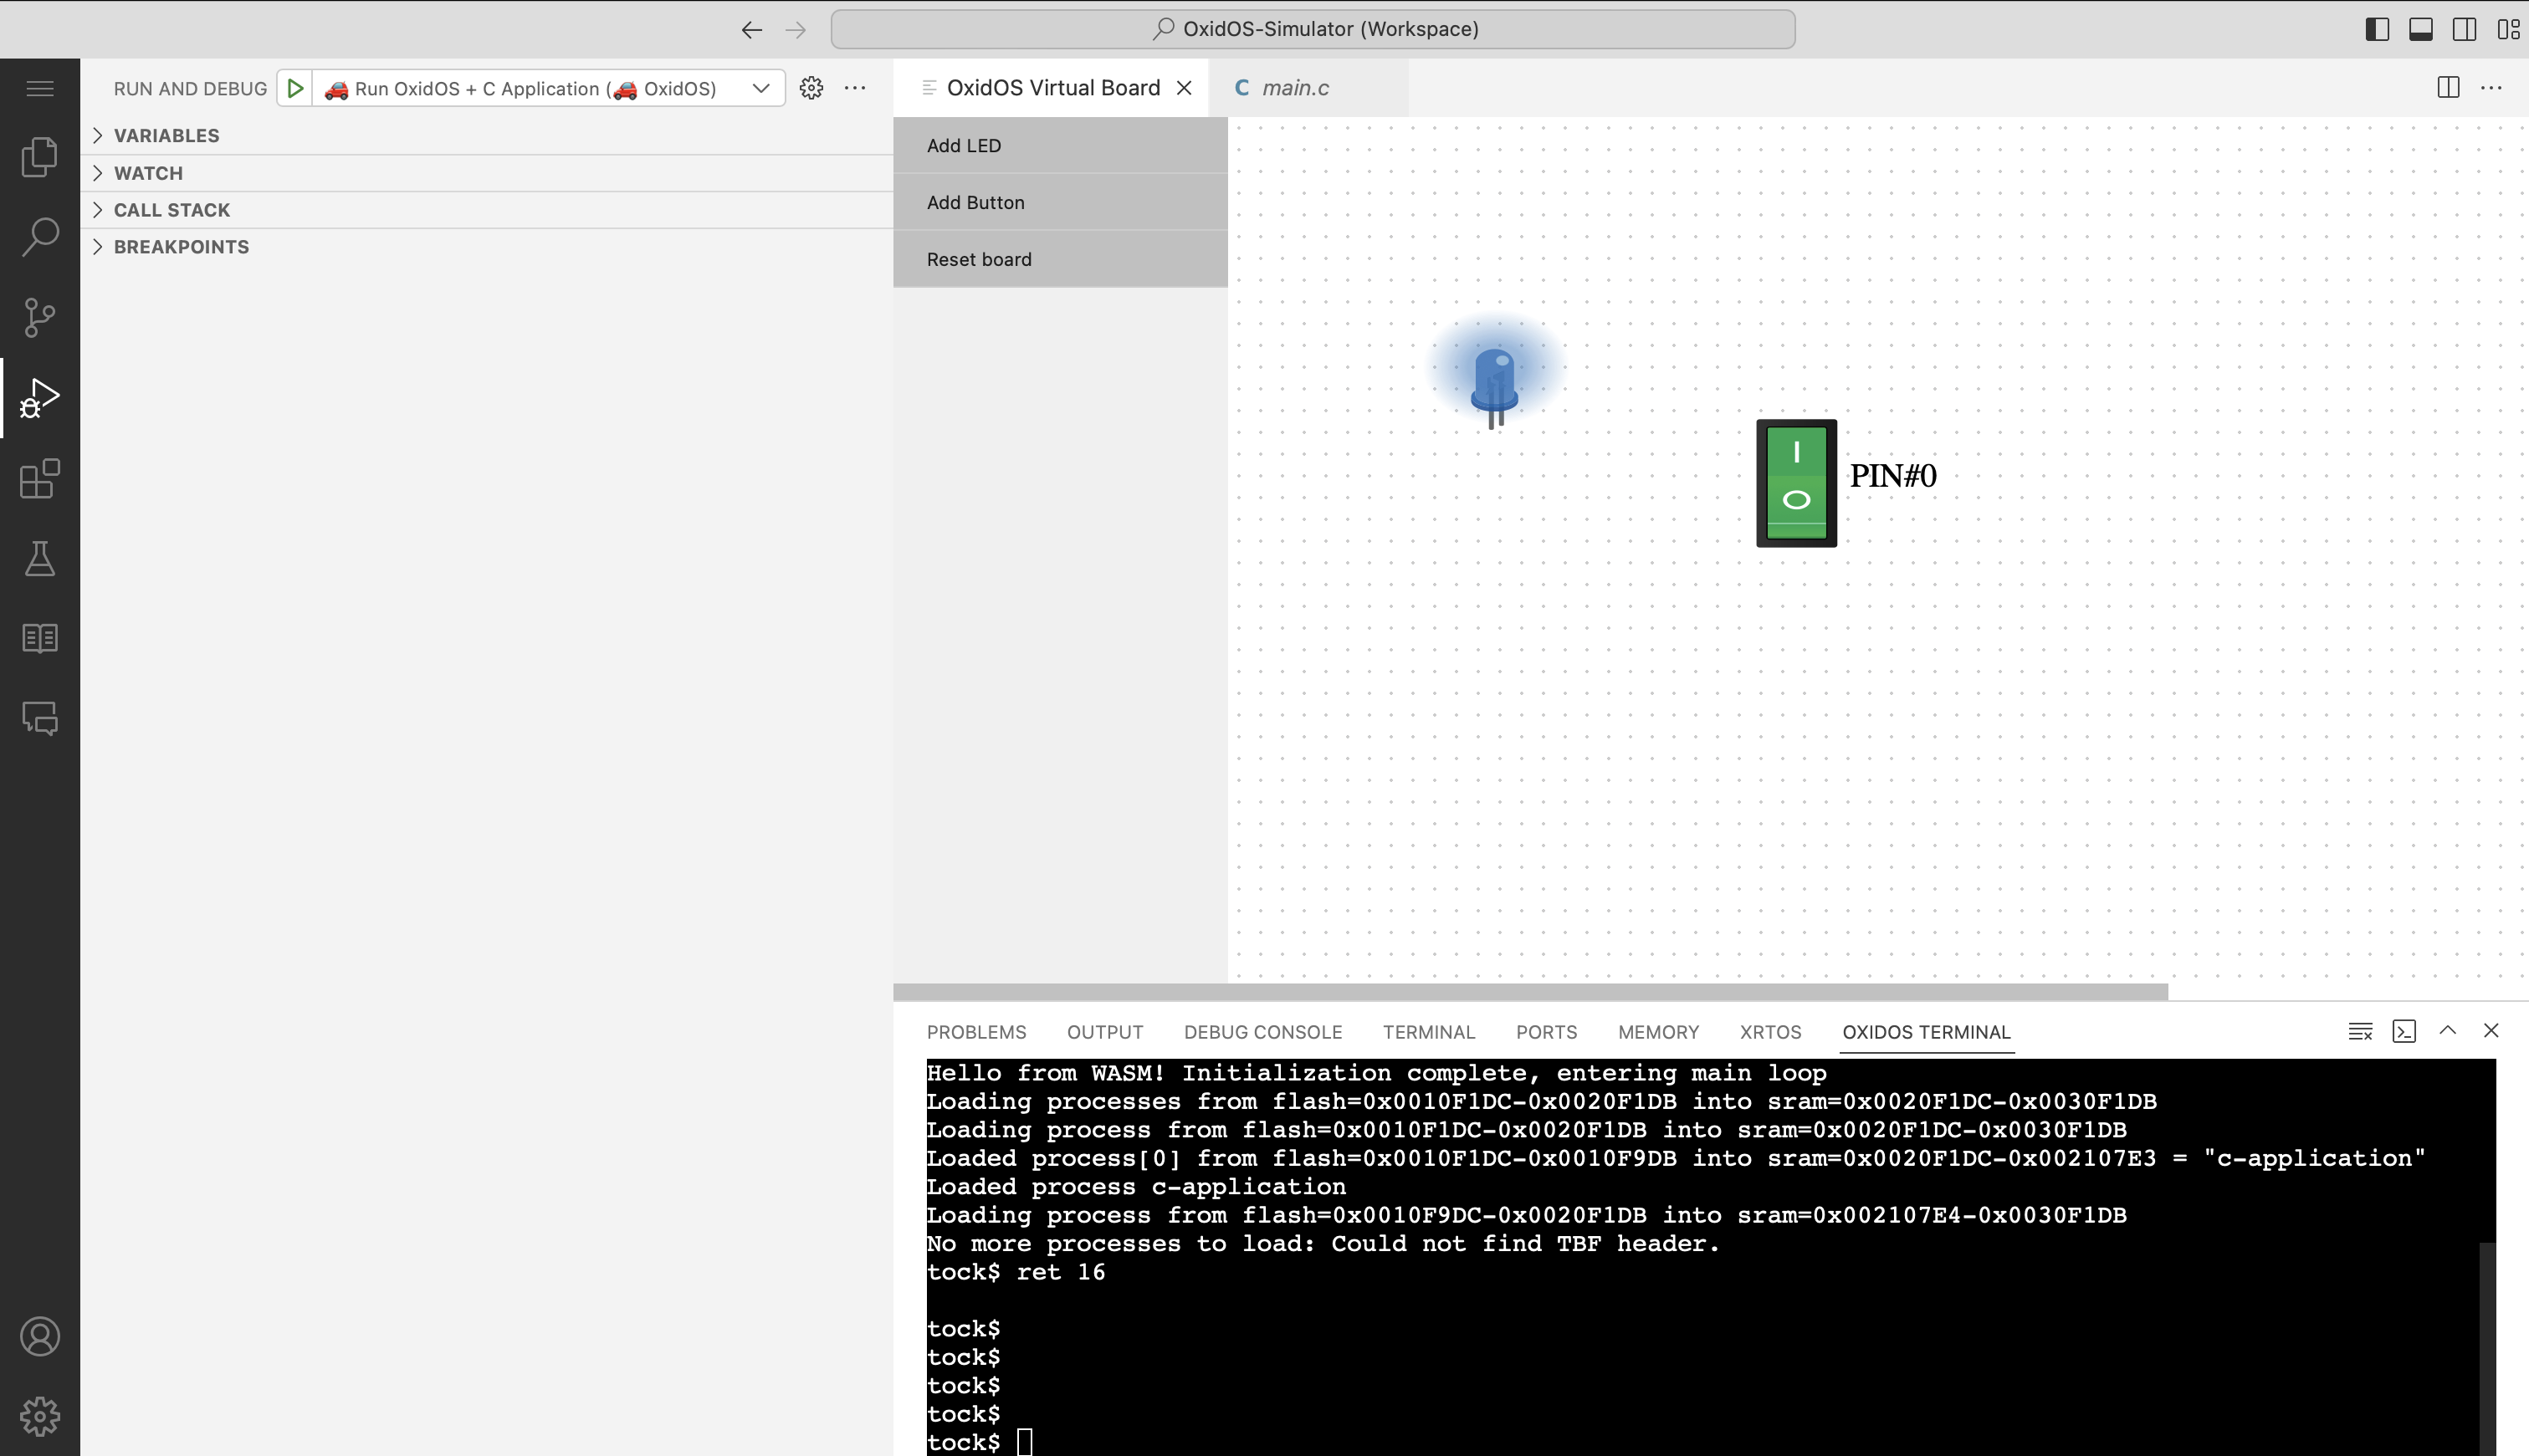
\includegraphics[scale=0.30]{pics/vscode_platform.png}
  \caption[C application communicating with simulated peripherals]{C application communicating with simulated peripherals}
  \label{fig:platform}
\end{figure}

\subsection{Userspace application and kernelspace debugger}

Visual Studio Code provides JSON-defined launch tasks in order to integrate a certain debugger to the development environment of a project.

For the userspace debugger to be validated, the debugger server must successfully connect to the text editor's Debug Adapter Protocol, so the debugging procedure can be visualised directly on the source code.

\begin{lstlisting}[language=GDB]
set remotetimeout 10
set architecture armv7e-m
set arm fallback-mode thumb
set debug remote 1
b main
\end{lstlisting}

For the GDB server to start the connection automatically, it has to run a script of commands to prepare the environment. This will facilitate the definition of the project's launch task.

The conditions were met when testing a the same C application used for testing the simulated peripheral, through setting breakpoints, stepping through code and viewing the internal variables' values inside the text editor.

\begin{figure}[H]
\centering
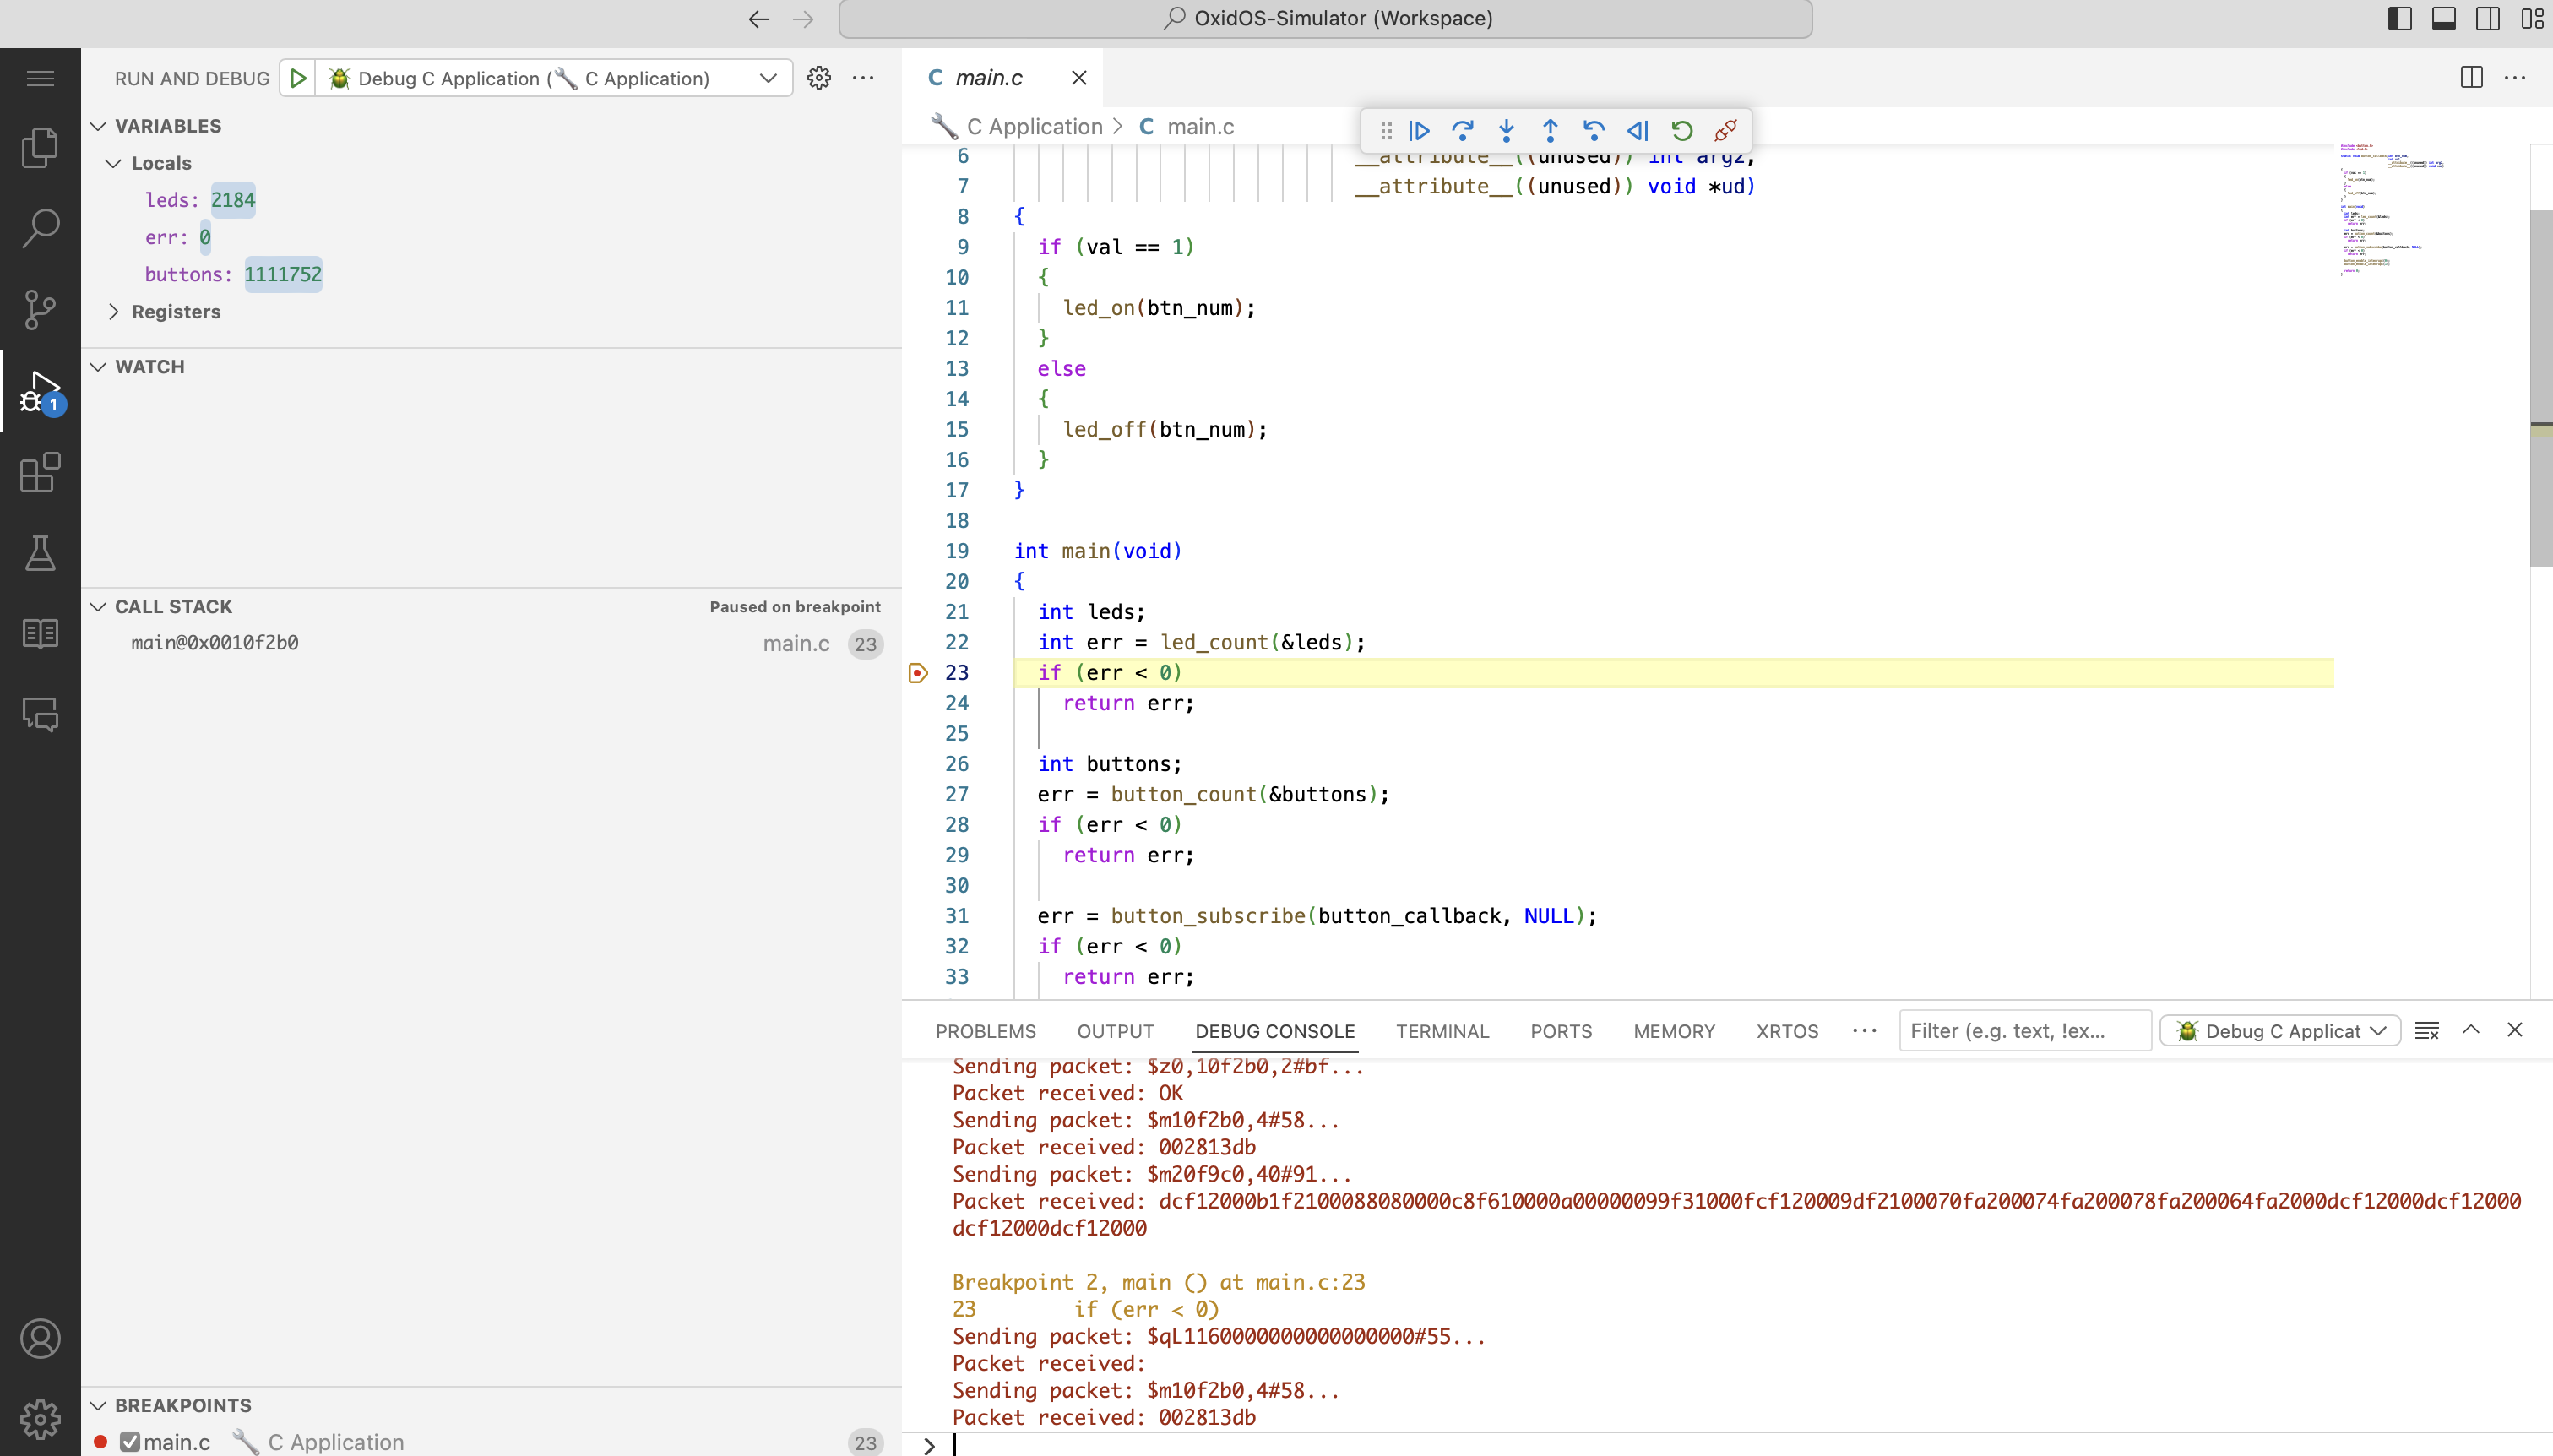
\includegraphics[scale=0.30]{pics/vscode_debug.png}
  \caption[C application being debugged]{C application being debugged}
  \label{fig:platform}
\end{figure}

\section{Testing}

Testing of the previously described platform was done in three sessions with groups of five to ten users. The first main bug encountered early on the project was the debugger's lag on both connecting to the Visual Studio Code extension and on stepping through code. This was fixed by removing the acknowledgment packages on the GDB server and increasing the remote timeout value to 10 seconds.

\chapter{Conclusions}

\chapter*{Bibliography}\addcontentsline{toc}{chapter}{Bibliography}  
% * <marios.choudary@gmail.com> 2018-02-28T12:07:48.730Z:
% 
% > BIBLIOGRAFIE
% Am adaugat un paragraf cu cateva detalii despre folosirea citarilor bibliografice in Latex, despre folosirea lui "\cite" si despre posibilitatea folosirii bibliografiei si direct in fisierul Latex.
% 
% ^.

\begin{itemize}
	\item 	NU utilizați referințe la Wikipedia sau alte surse fără autor asumat.
	\item 	Pentru referințe la articole relevante accesibile în web (descrise prin URL) se va nota la bibliografie și data accesării.
	\item 	Mai multe detalii despre citarea referințelor din internet se pot regăsi la:
	\begin{itemize}
		\item	\url{http://www.writinghelp-central.com/apa-citation-internet.html}
		\item	\url{http://www.webliminal.com/search/search-web13.html}
	\end{itemize}
	\item 	Note de subsol se utilizează dacă referiți un link mai puțin semnificativ o singură dată; Dacă nota este citată de mai multe ori, atunci utilizați o referință bibliografică.
	\item 	Dacă o imagine este introdusă în text și nu este realizată de către autorul lucrării, trebuie citată sursa ei (ca notă de subsol sau referință - este de preferat utilizarea unei note de subsol).
	\item 	Referințele se pun direct legate de text (de exemplu ``KVM [1] uses'', ``as stated by Popescu and Ionescu [12]'', etc.). Nu este recomandat să folosiți formulări de tipul ``[1] uses'', ``as stated in [12]'', ``as described in [11]'' etc..
	\item 	Afirmațiile de forma ``are numerous'', ``have grown exponentially'', ``are among the most used'', ``are an important topic'' trebuie să fie acoperite cu citări, date concrete si analize comparative.
	\begin{itemize}
		\item	Mai ales în capitolele de introducere, ``state of the art'', ``related work'' sau ``background'' trebuie să vă argumentați afirmațiile prin citări. Fiți autocritici și gândiți-vă dacă afirmațiile au nevoie de citări, chiar și cele pe care le considerați evidente.
		\item	Cea mai mare parte dintre citări vor fi în capitolele de introducere ``state of the art'', ``related work'' sau ``background''.
	\end{itemize}
	\item 	Toate intrările bibliografice trebuie citate în text. Nu le adăugați pur și simplu la final.
	\item 	Nu copiați sau traduceți niciodată din surse de informație de orice tip (online, offline, cărți, etc.). Dacă totuși doriți să oferiți, prin excepție, un citat celebru - de maxim 1 frază- utilizați ghilimele și evident menționați sursa. .
	\item 	Dacă reformulați idei sau creați un paragraf rezumat al unor idei folosind cuvintele voastre, precizați cu citare (referință bibliografică) sau cu notă de subsol sursa sau sursele de unde ați preluat ideile.
\end{itemize}

Trebuie respectat un singur standard de trimiteri bibliografice (citare), dintre următoarele alternative:
\begin{itemize}
	\item APA (\url{http://pitt.libguides.com/c.php?g=12108\&p=64730})
	\item IEEE (\url{https://ieee-dataport.org/sites/default/files/analysis/27/IEEE\%20Citation\%20Guidelines.pdf}) 
	\item Harvard (\url{https://libweb.anglia.ac.uk/referencing/harvard.htm})
	\item Cu numerotarea referințelor în ordine alfabetică sau în ordinea apariției în text (de exemplu, stilul cu numere folosit de unele publicații ACM - \url{https://www.acm.org/publications/authors/reference-formatting}) 
\end{itemize}

În Latex este foarte ușor să folosiți referințe într-un mod corect și unitar, fie prin adăugarea unei secțiuni
\verb!\begin{thebibliography}!
(vezi la sfârșitul acestei secțiuni), fie printr-un fișier separat de tip bib, folosind comanda
\verb!\bibliography{}!,
așa cum procedăm mai jos prin folosirea fișierului ``bibliography.bib''. În orice caz, în Latex va trebui să folosiți comanda
\verb!\cite{}!
pentru a adăuga referințe, iar această comandă trebuie folosită direct în text, acolo unde vreți sa apară citația, ca în exemplele următoare:
\begin{itemize}
	\item Articol jurnal: ~\cite{article};
	\item Articol conferință:~\cite{proc};
	\item Carte: ~\cite{book};
	\item Weblink: ~\cite{silva};
\end{itemize}

\textbf{Important}: în această secțiune de obicei apar doar intrările bibliografice (adică doar listarea referințelor). Citarea lor prin comanda cite și explicații legate de ele trebuie facute în secțiunile anterioare. Citarea de mai sus a fost facută aici doar pentru exemplificare.

% Asa se specifica folosirea unui fisier cu referinte bibliografice:
\bibliographystyle{plain}
\bibliography{bibliography}

%% O alta varianta ar fi fost includerea de articole direct in acest fisier
%% in felul urmator:
%% \begin{thebibliography}{ABC}
%%
%% \bibitem{article}
%%  H. Baali, H. Djelouat, A. Amira and F. Bensaali,
%%  ``Empowering Technology Enabled Care Using IoT and Smart Devices:
%   A Review''. In: IEEE Sensors Journal, vol. 322 (10), pp. 891--921, 1905.
%%
%% (more \bibitem items here...)
%%
%% \end{thebibliography}

%% Daca vreti ca o sectiune sa inceapa pe o pagina noua, puteti forta acest lucru cu comanda "\newpage", ca mai jos:

%\newpage

\chapter*{Anexe}\addcontentsline{toc}{chapter}{Anexe}

Anexele sunt opționale.
Ce poate intra în anexe:
\begin{itemize}
\item	Exemplu de fișier de configurare sau compilare;
\item	Un tabel mai mare de o jumătate pagină;
\item	O figura mai mare mai mare de jumătate pagină;
\item	O secvență de cod sursa mai mare de jumătate pagină;
\item	Un set de capturi de ecran (``screenshot''-uri);
\item	Un exemplu de rulare a unor comenzi plus rezultatul (``output''-ul) acestora;
\item 	În anexe intră lucruri care ocupă mai mult de o pagină ce ar întrerupe firul natural de parcurgere al textului.
\end{itemize}

\begin{appendices}

\chapter{Extrase de cod} % Introduce o nouă anexă
\ldots


\end{appendices}
\end{document}
